\section{Proposed methodology\label{sec:methodology}}

 In this section, we first adapt the privacy framework of $k-$anonymity to the case of graph data (\cref{sec:graph-k-anonymity}). Next we introduce our methodology: We assume that all mobility data are initially represented as a sequence of pseudonymous locations.
We also assume that the pseudonymisation process is distinct per user, and therefore locations cannot be compared between individuals.
In other words, it is not possible to determine whether pseudonymous location $l_u$ for user $u$ is the same as (or different from) location $l_v$ for user $v$.
We convert a location sequence for each user into a mobility network (\cref{sec:mobility-networks}). 
We then extract feature representations of these networks and embed them into a vector space.
Finally, in the vector space, we can define pairwise distances between the network embeddings (\cref{sec:graph-kernels}) and use them in a deanonymization scenario (\cref{sec:deanon-leakage}).  

Our methodology is, in principle, applicable to many other categories of recurrent behavioural trajectories that can be abstracted as graphs, such web browsing sessions~\citep{olejnik14, yen12} or smartphone application usage sequences~\citep{Welke2016}.

\subsection{$k-$anonymity on graphs\label{sec:graph-k-anonymity}}

Anonymity among networks refers to topological (or structural) equivalence. In our analysis we adopt the privacy framework of $k-$anonymity~\citep{sweeney2002k}, which we summarize as follows:

\ndefn[\textbf{$k-$anonymity}]{
	A microdata release of statistics, containing separate entries for a number of individuals in the population, satisfies the $k-$anonymity property, iff the information for each individual contained in the release is indistinguishable from at least $k-1$ other individuals whose information also appears in the release.
}

\vspace{.4cm}
Therefore we interpret $k-$anonymity in this chapter to mean that the mobility network of an individual in a population should be identical to the mobility network of at least $k-1$ other individuals.
Recent work casts doubt on the protection guarantees offered by \mbox{$k-$anonymity} in location privacy~\citep{shokri2010}, motivating the definition of $l-$diversity~\citep{Machanavajjhala2007} and $t-$closeness~\citep{li2007}.
Although $k-$anonymity may be insufficient to ensure privacy in the presence of adversarial knowledge, \mbox{$k-$anonymity} is a good metric to use to measure the uniqueness of an individual in the data.
Moreover, this framework is straightforwardly generalizable to the case of graph data.

Structural equivalence in the space of graphs corresponds to isomorphism and, based on this, we can define \emph{$k-$anonymity on unweighted graphs} as follows:

\ndefn[\textbf{Graph Isomorphism}]{
	Two graphs $ G=(V, E) $ and $ G'=(V', E') $ are \emph{isomorphic} (or \emph{belong to the same isomorphism class}) if there exists a bijective mapping $ g: V \rightarrow V' $ such that $ (v_i, v_j) \in E $ iff $ \left(g(v_i), g(v_j)\right) \in E'$.
}

\ndefn[\textbf{Graph $k-$anonymity}]{
 \emph{Graph} \mbox{$k-$\emph{anonymity}} is the minimum cardinality of isomorphism classes within a population of graphs.
}

\vspace{.4cm}
After clustering our population of graphs into isomorphism classes, we can also define the \emph{identifiability set} and \emph{anonymity size}~\citep{anon_terminology} as follows:

\ndefn[\textbf{Identifiability Set}]{
	\emph{Identifiability set} is the percentage of the population which is uniquely identified given their top$-N$ network.
}

\ndefn[\textbf{Anonymity Size}]{
	The \emph{anonymity size} of a network within a population is the cardinality of the isomorphism class to which the network belongs.
}

\subsection{Mobility information networks\label{sec:mobility-networks}}

To study the topological patterns of mobility, we represent user movements by a mobility network.
A preliminary step is to check whether a first-order network is a reasonable representation of movement data, or whether a higher-order network is required.

First-order network representations of mobility traces are built on the assumption of a \emph{first-order temporal correlation} among their states.
In the case of mobility data, this means that the transition by an individual to the next location in the mobility network can be accurately modelled by considering only their current location.
For example, the probability that an individual visits the shops or work next depends only on where they are located now, and a more detailed past history of places recently visited does not offer significant improvements to the model.
The alternative is that a sequence of the states is better modelled by higher-order Markov chains, namely that transitions depend on the current state and one or more previously visited states.
For example, the probability that an individual visits the shops or work next depends not only on where they are now, but where they were earlier in the day or week.
If higher-order Markov chains are required, we should assume a larger state-space and use these states as the nodes of our individual mobility networks.
Recently proposed methods on optimal order selection of sequential data~\citep{xu2016representing, scholtes2017network} can be directly applied at this step.

Let us assume a mobility dataset from a population of users $ u \in U$.
We introduce two network representations of user's mobility.

\ndefn[\textbf{State Connectivity Network}]{ 
A \textbf{state connectivity network} for $ u $ is an unweighted directed graph $ C^{u}=\left(V^{u}, E^{u}\right) $. Nodes $ v_i \in V^{u} $ correspond to states visited by the user throughout the observation period.  An edge $ e_{ij} = \left(v_i^u, v_j^u\right) \in E^{u} $ represents the information that $ u $ had at least one recorded transition from $ v_i^u $ to $ v_j^u $.
}

\ndefn[\textbf{Mobility Network}]{ 
A \textbf{mobility network} for $ u $ is a weighted and directed
graph $G^{u}=\left(V^{u}, E^{u}, W^{u}\right)  \in \mcG$, with the same topology as the state connectivity network and additionally an edge weight function $ W^{u} : E^{u} \rightarrow \mathbb{R}^{+}$. The weight function assigns a frequency $ w_{ij}^u $ to each edge $ e_{ij}^u $, which corresponds to the number of transitions from $ v_i^u  $ to $ v_j^u $ recorded throughout the observation period.
}

\vspace{.4cm}
To facilitate comparisons of frequencies across networks of different sizes in our experiments, we normalize edge weights on each mobility network to sum \mbox{to 1}.

In first-order networks, nodes correspond to distinct places that the user visits.
Given a high-frequency, timestamped sequence of location events for a user, distinct places can be extracted as small geographic regions where a user stays longer than a defined time interval, using existing clustering algorithms~\citep{kang2005extracting}.
Nodes in the mobility network have no geographic or timing information associated with them.
Nodes may have \emph{attributes} attached to them reflecting additional side information.
For example, in this study we consider whether attaching the frequency of visits a user makes to a specific node aids an attacker attempting to deanonymize the user.

In some of our experiments, we prune the mobility networks of users by reducing the size of the mobility network to the $ N $ most frequent places and rearranging the edges in the network accordingly.
We refer to these networks as \textbf{top$-N $ mobility networks}.

\subsection{Graph similarity metrics\label{sec:graph-kernels}}

It is not practical to apply a graph isomorphism test to two mobility networks to determine if they represent the same underlying user, because a user's mobility network is likely to vary over time.
Therefore we need distance functions that can measure the degree of similarity between two graphs.
Distance functions decompose the graph into feature vectors (smaller substructures and pattern counts), or histograms of graph statistics, and express similarity as the distance between those feature representations.
In the following, we introduce the notion of graph kernels and describe the graph similarity metrics used later in our experiments.

We wish to compute the similarity between two graphs $ G, G' \in \mcG$. 
To this end, according to the definitions of~\cref{subsec:b-kernels}, we will use graph kernel functions $ K(G, G') : \mcG \times \mcG \rightarrow \mcR^{+}$~\citep{Vishwanathan2010}, and their corresponding feature maps $\phi(G)$.


In order to ensure the result from the kernel lies in the interval $[-1, 1]$, we apply \emph{cosine normalization} as follows:
\[
K({G}, {G}')=\left  \langle \frac{\phi({G})}{||\phi({G})||}, \frac{\phi(G')}{||\phi(G')||} \right  \rangle.
\]
One interpretation of this function is as the \emph{cosine similarity of the graphs in the feature space} defined by the map of the kernel.

In our experiments we apply a number of kernel functions on our mobility datasets and assess their suitability for deanonymization applications on mobility networks.
We note in advance that, as the degree distribution and all substructure counts of a graph remain unchanged under structure-preserving bijection of the vertex set, all examined graph kernels are invariant under isomorphism.
We briefly introduce these kernels in the remainder of the section.


\subsubsection{Kernels on degree distribution }

The degree distribution of nodes in the graph can be used to quantify the similarity between two graphs.
For example, we can use a histogram of weighted or unweighted node degree as a feature vector.
We can then compute the pairwise distance of two graphs by taking either the inner product of the feature vectors, or passing them through a Gaussian Radial Basis Function kernel:
\[ K(G,G') =\exp\left( -\frac{||\phi(G) - \phi(G')||^2}{2\sigma^2} \right).\]
Here, the hyperparameters of the kernel are the variance $\sigma$~(in case RBF is used), and the number of bins in the histogram.

\subsubsection{Kernels on graph atomic substructures}

Kernels can use counts on substructures, such as subtree patterns, shortest paths, walks, or limited-size subgraphs.
This family of kernels are called \emph{$R-$convolution graph kernels}~\citep{haussler}.
In this way, graphs are represented as vectors with elements corresponding to the frequency of each such substructure over the graph.
Hence, if
$ s_1, s_2, ... \in \mcS$ are the substructures of interest and $ \#\left(s_i \in G\right)$ the counts of $ s_i $ in graph $ G $, we get as feature map vectors
\[ 
\phi(G) = \left[\#\left(s_1 \in G\right), \#\left(s_2 \in G\right), \dots\right]^T
\label{eq:rconv-features}
\]
with dimension $ |\mcS| $  and kernel
\[
K(G, G') = \sum_{s \in \mathcal{S}} \#\left(s \in G\right) \#\left(s \in G'\right).
\]

In the following, we briefly present some kernels in this category and explain how they are adapted in our experiments.

\vspace{1em}
\noindent\textbf{Shortest-Path Kernel}

The Shortest-Path (\emph{SP}) graph kernel~\citep{borgwardt2005} expresses the similarity between two graphs by counting the co-occurring shortest paths in the graphs.
It can be written in the form of~\cref{eq:rconv-features}, where each element $ s_i \in \mcS $ is a triplet $\big(a_{\text{start}}^i, a_{\text{end}}^i, n\big)$, where $ n $ is the length of the path and $ a_{\text{start}}^i, a_{\text{end}}^i $ the attributes of the starting and ending nodes.
The shortest path set is computable in polynomial time using, for example, the Floyd-Warshall algorithm, with complexity $ O(|V|^4)$, where $ |V| $ is number of nodes in the network.

\vspace{1em}
\noindent\textbf{Weisfeiler-Lehman Subtree Kernel}

\begin{figure*}[t]
	%\includegraphics[totalheight=7.3cm]{fig/wl_graph1_tikz.png}
	\centering 
	\begin{subfigure}[t]{.19\textwidth}
		\resizebox{0.6\textwidth}{0.08\textheight}{%
			\centering 
			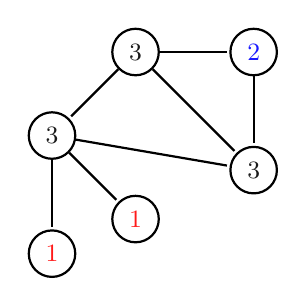
\begin{tikzpicture}[shorten >=1pt, thick, auto,node distance=1.5cm,font=\small]
			\tikzstyle{state1}=[circle,draw=black,text=red!90, font=\small]
			\tikzstyle{state2}=[circle,draw=black,text=blue!90!, font=\small]
			\tikzstyle{state3}=[circle,draw=black, text=black!90,  font=\small]
			\tikzstyle{state4}=[circle,draw=black, text={rgb:red,1;green,2;blue,3},  maximum size=0.5cm,font=\small]
			\tikzstyle{state5}=[circle,draw=black, text=green!90!black!,  maximum size=0.5cm,font=\small]
			\tikzstyle{state6}=[circle,draw=black, text=black!90,  maximum size=0.5cm,font=\small]
			\tikzstyle{state7}=[circle,draw=black, text=red!,  maximum size=0.5cm, font=\small]
			\tikzstyle{state8}=[circle,draw=black,text=black!50!blue!,  maximum size=0.5cm,font=\small]
			\tikzstyle{state9}=[circle, draw=black,text=orange!90,  maximum size=0.5cm,font=\small]
			\node[state3] 		 (A0)                    {$3$};
			\node[state2]         (B0) [right of=A0 ] {$2$};
			\node[state3]         (C0) [below left of=A0] {$3$};
			\node[state3]         (D0) [below  of=B0] {$3$};
			\node[state1]         (E0) [below  of=C0] {$1$};
			\node[state1]         (F0) [below  right of=C0] {$1$};
			\draw (A0) edge[thick]  (B0);
			\draw (B0) edge[thick] (D0);
			\draw (A0) edge[thick]  (D0);
			\draw (A0) edge[thick] (C0);
			\draw (C0) edge[thick]  (D0);
			\draw (C0) edge[thick] (E0);
			\draw (C0) edge[thick]  (F0);
			\end{tikzpicture}}
		\caption{$G$} \label{fig:G}
	\end{subfigure}
	\centering 
	\begin{subfigure}[t]{.19\textwidth}
		\resizebox{0.6\textwidth}{0.08\textheight}{%
			\centering
			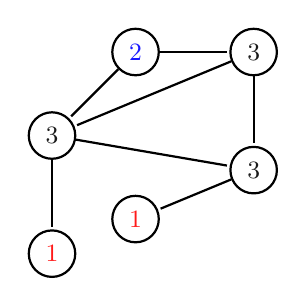
\begin{tikzpicture}[shorten >=1pt, thick, auto,node distance=1.5cm]
			\tikzstyle{state1}=[circle,draw=black,text=red!90, font=\small]
			\tikzstyle{state2}=[circle,draw=black,text=blue!90!, font=\small]
			\tikzstyle{state3}=[circle,draw=black, text=black!90,  font=\small]
			\tikzstyle{state4}=[circle,draw=black, text={rgb:red,1;green,2;blue,3},  maximum size=0.5cm,font=\small]
			\tikzstyle{state5}=[circle,draw=black, text=green!90!black!,  maximum size=0.5cm,font=\small]
			\tikzstyle{state6}=[circle,draw=black, text=black!90,  maximum size=0.5cm,font=\small]
			\tikzstyle{state7}=[circle,draw=black, text=red!,  maximum size=0.5cm, font=\small]
			\tikzstyle{state8}=[circle,draw=black,text=black!50!blue!,  maximum size=0.5cm,font=\small]
			\tikzstyle{state9}=[circle, draw=black,text=orange!90,  maximum size=0.5cm,font=\small]
			\node[state2] 		  (A1)                   {$2$};
			\node[state3]         (B1) [right of=A1] {$3$};
			\node[state3]         (C1) [below left of=A1]{$3$};
			\node[state3]         (D1) [below  of=B1] {$3$};
			\node[state1]         (E1) [below of=C1]        {$1$};
			\node[state1]         (F1) [below right of=C1]       {$1$};
			\draw (A1) edge[thick]  (B1);
			\draw (A1) edge[thick]  (C1);
			\draw (B1) edge[thick]  (C1);
			\draw (B1) edge[thick]  (D1);
			\draw (C1) edge[thick]  (D1);
			\draw (C1) edge[thick]  (E1);
			\draw (D1) edge[thick]  (F1);
			\end{tikzpicture}
		}
		\caption{$G'$} \label{fig:G'}
	\end{subfigure}
	\centering 
	\begin{subfigure}[t]{.19\textwidth}
		\resizebox{0.6\textwidth}{0.08\textheight}{%
			\centering 
			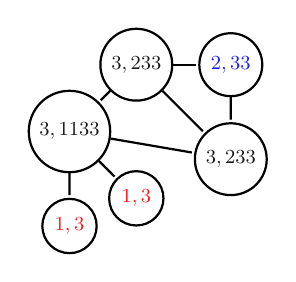
\begin{tikzpicture}[shorten >=1pt, thick, auto,node distance=1.5cm,font=\small]
			\tikzstyle{state1}=[circle,draw=black,text=red!90,scale=0.8, font=\small]
			\tikzstyle{state2}=[circle,draw=black,text=blue!90!,scale=0.8, font=\small]
			\tikzstyle{state3}=[circle,draw=black, text=black!90,  scale=0.8,font=\small]
			\tikzstyle{state4}=[circle,draw=black, text={rgb:red,1;green,2;blue,3},  maximum size=0.5cm,scale=0.8,font=\small]
			\tikzstyle{state5}=[circle,draw=black, text=green!90!black!,  maximum size=0.5cm,scale=0.8,font=\small]
			\tikzstyle{state6}=[circle,draw=black, text=black!90,  maximum size=0.5cm,scale=0.8,font=\small]
			\tikzstyle{state7}=[circle,draw=black, text=red!,  maximum size=0.5cm, scale=0.8,font=\small]
			\tikzstyle{state8}=[circle,draw=black,text=black!50!blue!,  maximum size=0.5cm,scale=0.8,font=\small]
			\tikzstyle{state9}=[circle, draw=black,text=orange!90,  maximum size=0.5cm,scale=0.8,font=\small]
			\node[state3] 		 (A0)                    {$3,233$};
			\node[state2]         (B0) [right of=A0 ] {$2,33$};
			\node[state3]         (C0) [below left of=A0] {$3,1133$};
			\node[state3]         (D0) [below  of=B0] {$3,233$};
			\node[state1]         (E0) [below  of=C0] {$1,3$};
			\node[state1]         (F0) [below right of=C0] {$1,3$};
			\draw (A0) edge[thick]  (B0);
			\draw (B0) edge[thick] (D0);
			\draw (A0) edge[thick]  (D0);
			\draw (A0) edge[thick] (C0);
			\draw (C0) edge[thick]  (D0);
			\draw (C0) edge[thick] (E0);
			\draw (C0) edge[thick]  (F0);
			\end{tikzpicture}}
		\caption{\mbox{$G$ with multiset} \mbox{node attributes}} \label{fig:Gmult}
	\end{subfigure}
	\centering 
	\begin{subfigure}[t]{.19\textwidth}
		\resizebox{0.6\textwidth}{0.08\textheight}{%
			\centering 
			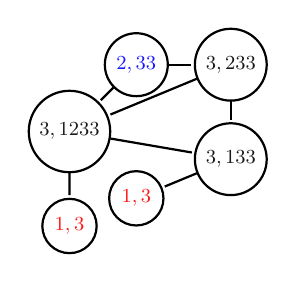
\begin{tikzpicture}[shorten >=1pt, thick, auto,node distance=1.5cm]
			\tikzstyle{state1}=[circle,draw=black,text=red!90,scale=0.8, font=\small]
			\tikzstyle{state2}=[circle,draw=black,text=blue!90!,scale=0.8, font=\small]
			\tikzstyle{state3}=[circle,draw=black, text=black!90,  scale=0.8,font=\small]
			\tikzstyle{state4}=[circle,draw=black, text={rgb:red,1;green,2;blue,3},  maximum size=0.5cm,scale=0.8,font=\small]
			\tikzstyle{state5}=[circle,draw=black, text=green!90!black!,  maximum size=0.5cm,scale=0.8,font=\small]
			\tikzstyle{state6}=[circle,draw=black, text=black!90,  maximum size=0.5cm,scale=0.8,font=\small]
			\tikzstyle{state7}=[circle,draw=black, text=red!,  maximum size=0.5cm, scale=0.8,font=\small]
			\tikzstyle{state8}=[circle,draw=black,text=black!50!blue!,  maximum size=0.5cm,scale=0.8,font=\small]
			\tikzstyle{state9}=[circle, draw=black,text=orange!90,  maximum size=0.5cm,scale=0.8,font=\small]
			\node[state2] 		  (A1)                   {$2,33$};
			\node[state3]         (B1) [right of=A1] {$3,233$};
			\node[state3]         (C1) [below left of=A1]{$3,1233$};
			\node[state3]         (D1) [below  of=B1] {$3,133$};
			\node[state1]         (E1) [below  of=C1]        {$1,3$};
			\node[state1]         (F1) [below right of=C1]       {$1,3$};
			\draw (A1) edge[thick]  (B1);
			\draw (A1) edge[thick]  (C1);
			\draw (B1) edge[thick]  (C1);
			\draw (B1) edge[thick]  (D1);
			\draw (C1) edge[thick]  (D1);
			\draw (C1) edge[thick]  (E1);
			\draw (D1) edge[thick]  (F1);
			\end{tikzpicture}}
		\caption{\mbox{$G'$ with multiset} \mbox{node attributes}} \label{fig:G'mult}
	\end{subfigure}
	\centering 
	\begin{subfigure}[t]{.19\textwidth}
		\centering 
		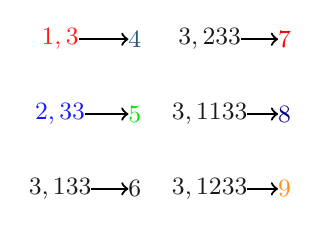
\begin{tikzpicture}[->, thick, auto,node distance=0.005cm,every node/.style={inner sep=0,outer sep=0}]
		\tikzstyle{state1}=[draw=white,text=red!90, font=\small]
		\tikzstyle{state2}=[draw=white,text=blue!90!, font=\small]
		\tikzstyle{state3}=[draw=white, text=black!90,  font=\small]
		\tikzstyle{state4}=[draw=white, text={rgb:red,1;green,2;blue,3},font=\small]
		\tikzstyle{state5}=[draw=white, text=green!90!black!,font=\small]
		\tikzstyle{state6}=[draw=white, text=black!90,  font=\small]
		\tikzstyle{state7}=[draw=white, text=red!,   font=\small]
		\tikzstyle{state8}=[draw=white,text=black!50!blue!,  font=\small]
		\tikzstyle{state9}=[ draw=white,text=orange!90,  font=\small]
		\begin{scope}[node distance=9.5mm and 0.1mm]
		\node[state1] 		  (A3)        {$1,3$};
		\node[state4] 		  (A4) [right  of = A3]   {$ 4 $};
		\node[state2]         (B3) [below of =A3] {$ 2,33 $};
		\node[state5]         (B4) [right  of =B3] {$ 5 $};
		\node[state3]         (C3) [below  of  =B3]{$ 3,133 $};
		\node[state6]         (C4) [right of = C3]{$ 6 $};
		\node[state3]         (D3) [right  of =A4]{$ 3,233 $};
		\node[state3]         (E3) [right  of  =B4] {$ 3,1133 $};
		\node[state3]         (F3) [right of = C4]  {$ 3,1233 $};
		\node[state7]         (D4) [right of = D3]{$ 7 $};
		\node[state8]         (E4) [right  of =E3] {$ 8 $};
		\node[state9]         (F4) [right of =F3] {$ 9 $};
		\draw (A3) edge[thick]  (A4);
		\draw (B3) edge[thick]  (B4);
		\draw (C3) edge[thick]  (C4);
		\draw (D3) edge[thick]  (D4);
		\draw (E3) edge[thick]  (E4);
		\draw (F3) edge[thick]  (F4);
		\end{scope}
		\end{tikzpicture}
		\caption{\mbox{Label Compression}} \label{fig:mapping}
	\end{subfigure}
	
	\medskip
	\centering 
	\begin{subfigure}[t]{.2\textwidth}
		\resizebox{0.6\textwidth}{0.08\textheight}{%
			\centering 
			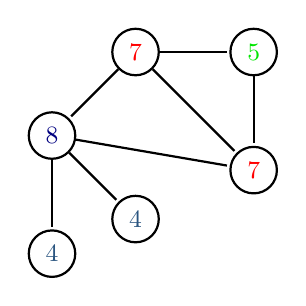
\begin{tikzpicture}[shorten >=1pt, thick, auto,node distance=1.5cm,font=\small]
			\tikzstyle{state1}=[circle,draw=black,text=red!90, font=\small]
			\tikzstyle{state2}=[circle,draw=black,text=blue!90!, font=\small]
			\tikzstyle{state3}=[circle,draw=black, text=black!90,  font=\small]
			\tikzstyle{state4}=[circle,draw=black, text={rgb:red,1;green,2;blue,3},  font=\small]
			\tikzstyle{state5}=[circle,draw=black, text=green!90!black!,  font=\small]
			\tikzstyle{state6}=[circle,draw=black, text=black!90,  font=\small]
			\tikzstyle{state7}=[circle,draw=black, text=red!, font=\small]
			\tikzstyle{state8}=[circle,draw=black,text=black!50!blue!,  font=\small]
			\tikzstyle{state9}=[circle, draw=black,text=orange!90,  font=\small]
			\node[state7] 		 (A0)                    {$7$};
			\node[state5]         (B0) [right of=A0 ] {$5$};
			\node[state8]         (C0) [below left of=A0] {$8$};
			\node[state7]         (D0) [below  of=B0] {$7$};
			\node[state4]         (E0) [below  of=C0] {$4$};
			\node[state4]         (F0) [below  right of=C0] {$4$};
			\draw (A0) edge[thick]  (B0);
			\draw (B0) edge[thick] (D0);
			\draw (A0) edge[thick]  (D0);
			\draw (A0) edge[thick] (C0);
			\draw (C0) edge[thick]  (D0);
			\draw (C0) edge[thick] (E0);
			\draw (C0) edge[thick]  (F0);
			\end{tikzpicture}
		}
		\caption{{$G$ relabeled}} \label{fig:Grel}
	\end{subfigure}
	\centering 
	\begin{subfigure}[t]{.2\textwidth}
		\resizebox{0.6\textwidth}{0.08\textheight}{%
			\centering 
			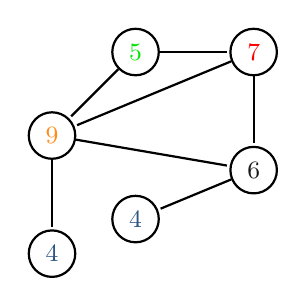
\begin{tikzpicture}[shorten >=1pt, thick, auto,node distance=1.5cm]
			\tikzstyle{state1}=[circle,draw=black,text=red!90, font=\small]
			\tikzstyle{state2}=[circle,draw=black,text=blue!90!, font=\small]
			\tikzstyle{state3}=[circle,draw=black, text=black!90,  font=\small]
			\tikzstyle{state4}=[circle,draw=black, text={rgb:red,1;green,2;blue,3},  font=\small]
			\tikzstyle{state5}=[circle,draw=black, text=green!90!black!, font=\small]
			\tikzstyle{state6}=[circle,draw=black, text=black!90,  font=\small]
			\tikzstyle{state7}=[circle,draw=black, text=red!,   font=\small]
			\tikzstyle{state8}=[circle,draw=black,text=black!50!blue!,  font=\small]
			\tikzstyle{state9}=[circle, draw=black,text=orange!90,  font=\small]
			\node[state5] 		  (A1)                   {$5$};
			\node[state7]         (B1) [right of=A1] {$7$};
			\node[state9]         (C1) [below left of=A1]{$9$};
			\node[state6]         (D1) [below  of=B1] {$6$};
			\node[state4]         (E1) [below of=C1]        {$4$};
			\node[state4]         (F1) [below right of=C1]       {$4$};
			\draw (A1) edge[thick]  (B1);
			\draw (A1) edge[thick]  (C1);
			\draw (B1) edge[thick]  (C1);
			\draw (B1) edge[thick]  (D1);
			\draw (C1) edge[thick]  (D1);
			\draw (C1) edge[thick]  (E1);
			\draw (D1) edge[thick]  (F1);
			\end{tikzpicture}
		}
		\caption{$G'$ relabeled} \label{fig:G'rel}
	\end{subfigure}
	\centering
	\begin{subfigure}[t]{.57\textwidth}
		\centering
		\begin{tikzpicture}[->, thick, auto,node distance=0.9cm,every node/.style={inner sep=0,outer sep=0}]
		\tikzstyle{state0}=[draw=white,text=black!, font=\small]
		\tikzstyle{state1}=[draw=white,text=red!90, font=\small]
		\tikzstyle{state2}=[draw=white,text=blue!90!, font=\small]
		\tikzstyle{state3}=[draw=white, text=black!90,  font=\small]
		\tikzstyle{state4}=[draw=white, text={rgb:red,1;green,2;blue,3},  font=\small]
		\tikzstyle{state5}=[draw=white, text=green!90!black!,  font=\small]
		\tikzstyle{state6}=[draw=white, text=black!90,  font=\small]
		\tikzstyle{state7}=[draw=white, text=red!,   font=\small]
		\tikzstyle{state8}=[draw=white,text=black!50!blue!,  font=\small]
		\tikzstyle{state9}=[ draw=white,text=orange!90,  font=\small]
		\begin{scope}[node distance=5.5mm and 3mm]
		\node[state0] 		  (O5)        {$  \mbox{features}$};
		\node[state1] 		  (A5)     [right=of  O5]    {$     1$};
		\node[state2]         (B5) [right=of A5] {$2$};
		\node[state3]         (C5) [right=of B5]{$3$};
		\node[state4]         (D5) [right=of C5]{$4$};
		\node[state5]         (E5) [right=of D5] {$5$};
		\node[state6]         (F5) [right=of E5] {$6$};
		\node[state7] 		  (G5) [right=of F5] {$7$};
		\node[state8]         (H5) [right=of G5] {$8$};
		\node[state9]         (I5) [right=of H5]{$9$};
		\node[state0] 		  (O6)    [below of=O5]{$\phi_1(G)=$};
		\node[state0] 		  (A6) [below of=A5] {$[2,$};
		\node[state0]         (B6) [below of=B5] {$1,$};
		\node[state0]         (C6) [below of=C5]{$3,$};
		\node[state0]         (D6) [below of=D5]{$2,$};
		\node[state0]         (E6) [below of=E5] {$1,$};
		\node[state0]         (F6) [below of=F5] {$0,$};
		\node[state0] 		  (G6) [below of=G5] {$2,$};
		\node[state0]         (H6) [below of=H5] {$1,$};
		\node[state0]         (I6) [below of=I5]{$0\;]$};
		\node[state0] 		  (O7)    [below of=O6] {$\phi_1(G')=$};
		\node[state0] 		  (A7)    [below of=A6]{$[2,$};
		\node[state0]         (B7) [below of=B6] {$1,$};
		\node[state0]         (C7) [below of=C6]{$3,$};
		\node[state0]         (D7) [below of=D6]{$2,$};
		\node[state0]         (E7) [below of=E6] {$1,$};
		\node[state0]         (F7) [below of=F6] {$1,$};
		\node[state0] 		  (G7) [below of=G6] {$1,$};
		\node[state0]         (H7) [below of=H6] {$0,$};
		\node[state0]         (I7) [below of=I6]{$1\;]$};
		\end{scope}
		\end{tikzpicture}
		\caption{extracted feature vectors} \label{fig:feat_G}
	\end{subfigure}
	
	\caption{{Computation of the Weisfeiler-Lehman subtree kernel of height $ h=1 $ for two attributed graphs.}}
	\label{fig:WL}
\end{figure*}


\textcite{Shervashidze2011} proposed an efficient method to construct a graph kernel utilizing the \mbox{Weisfeiler-Lehman} (\emph{WL}) test of isomorphism~\citep{weisfeiler1968reduction}.
The idea of the \emph{WL} kernel is to measure co-occurrences of subtree patterns across node attributed graphs.

Computation progresses over iterations as follows:
%
\begin{enumerate}
	\item each node attribute is augmented with a multiset of attributes from adjacent nodes;
	\item each node attribute is then compressed into a single attribute label for the next iteration; and
	\item the above steps are repeated until a specified threshold $ h $ is reached.
\end{enumerate}
%
An example is shown in~\cref{fig:WL}.

If $ G $ and $ G' $ are the two graphs, the \emph{WL} subtree kernel is defined as follows:
\[
K^{h}_{WL}(G, G') = \big \langle \phi_h(G), \phi_h(G') \big \rangle,
\]
where $ \phi_h(G) $ and $ \phi_h(G') $ are the vectors of labels extracted after running $ h $ steps of the computation (\cref{fig:feat_G}). They consist of $ h $ blocks, where the $i$-th component of the $j$-th block corresponds to the frequency of label $ i $ at the $j$-th iteration of the computation.
The computational complexity of the kernel scales \emph{linearly} with the number of edges $ |E| $ and the length $ h $ of the WL graph sequence.

\vspace{1em}
\noindent\textbf{Deep Graph Kernels}

Deep graph kernels (\emph{DK}s) are a unified framework that takes into account similarity relations at the level of atomic substructures in the kernel computation~\citep{yanardagV15}.
Hence, these kernels can quantify \emph{similar substructure} co-occurrence, offering more robust feature representations.
DKs are based on computing the following inner product:
\[
K(G, G') = \phi\left(G\right)^T M \phi\left(G'\right),
\]
where $ \phi $ is the feature mapping of a classical R-convolution graph kernel.

In the above, $M : |\mcV| \times |\mcV|$ is a positive semidefinitive matrix encoding the relationships between the atomic substructures and $ \mcV $ is the vocabulary of the observed substructures in the dataset.
Here, $ M $ can be defined using the edit distance of the substructures, i.e.\ the number of elementary operations to transform one substructure to another; or $ M $ can be learnt from the data, applying relevant neural language modeling methods \citep{mikolov2013efficient}.

\subsection{Deanonymization of user mobility networks and privacy leakage evaluation\label{sec:deanon-leakage}}

\subsubsection{Hypothesis}

\begin{figure}[!t]
	\centering
	\begin{subfigure}[]{0.495\textwidth}
		\centering		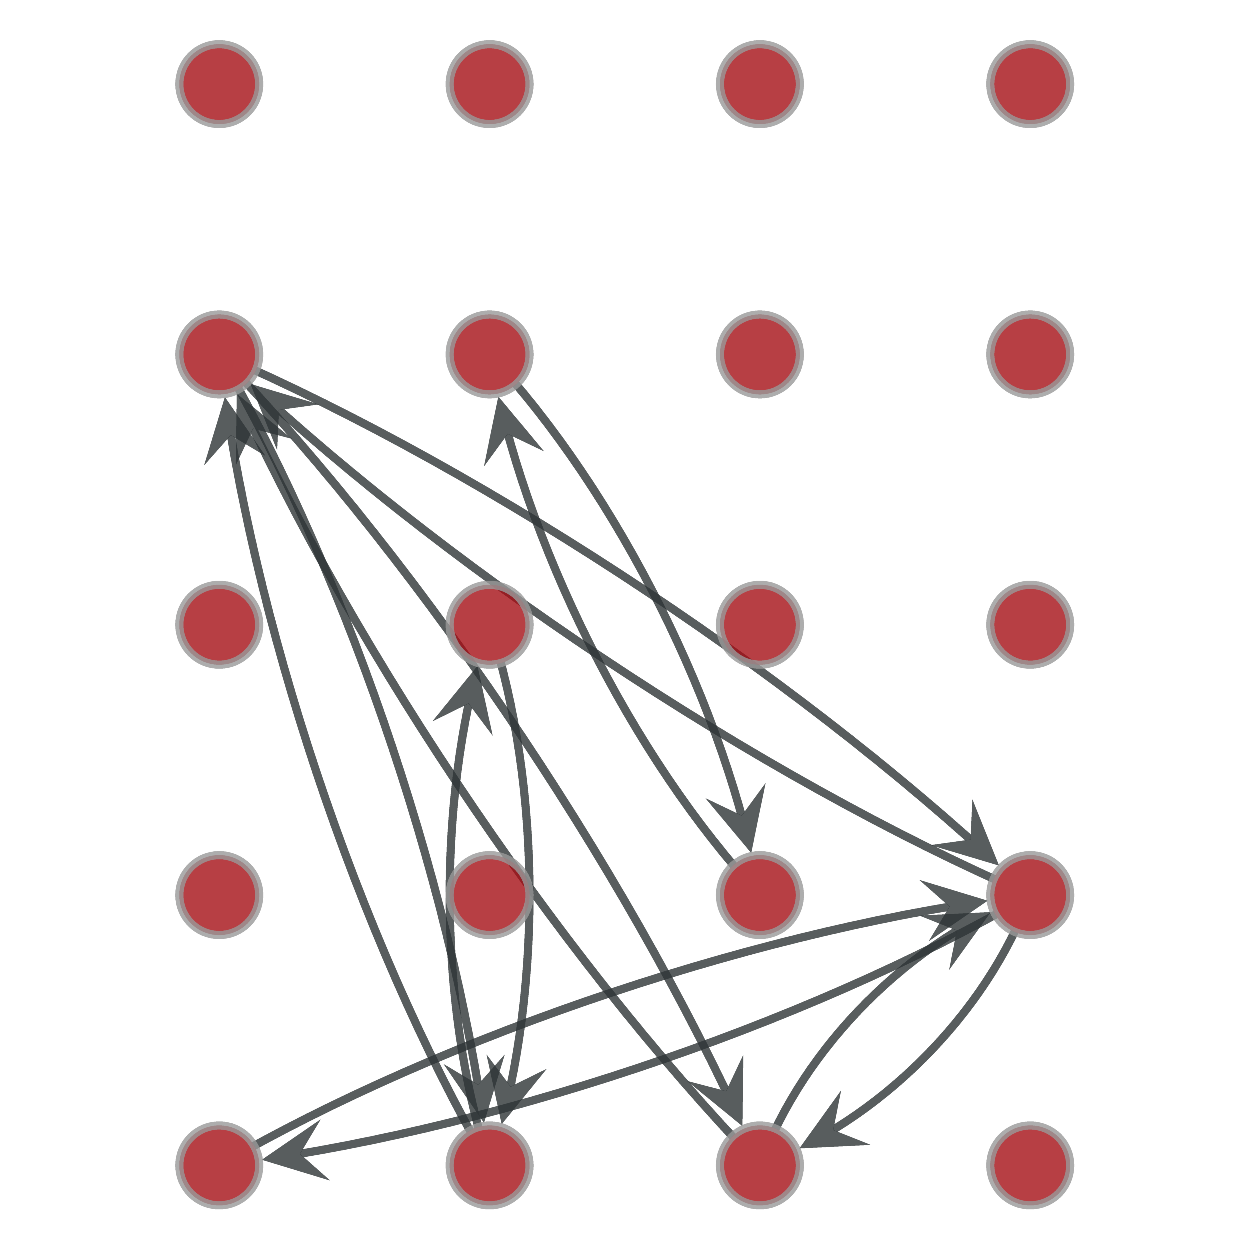
\includegraphics[height=4cm]{\MyPath/fig/1_firsthalf_.pdf}
		\caption{{\textbf{user 1}: 1\textsuperscript{st} half of the \mbox{observation period}}}
		\label{fig:evidence11}
	\end{subfigure}%
	\begin{subfigure}[]{0.495\textwidth}
		\centering
		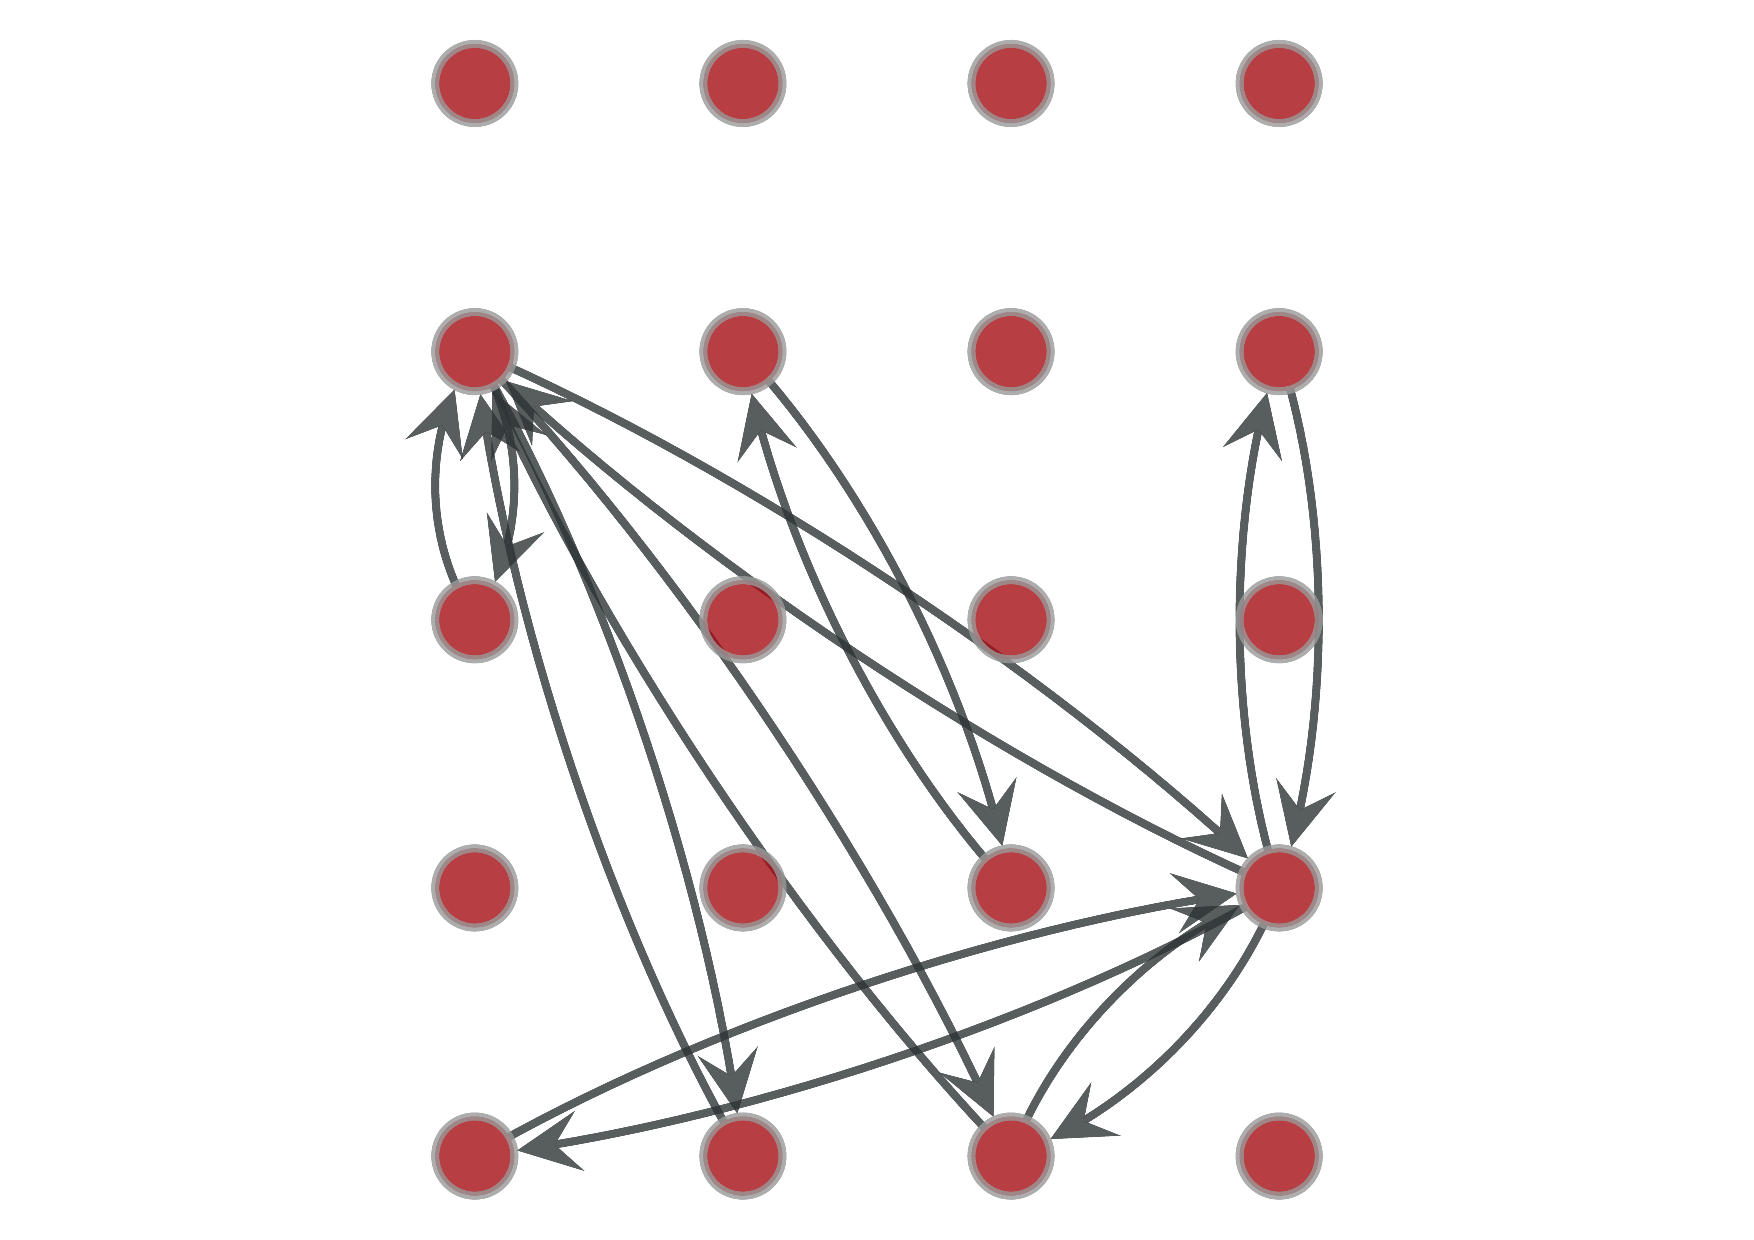
\includegraphics[height=4cm]{\MyPath/fig/1_secondhalf_.pdf}
		\caption{{\textbf{user 1}: 2\textsuperscript{nd} half of the \mbox{observation period}}}
		\label{fig:evidence12}
	\end{subfigure}%
	\\
	\begin{subfigure}[]{0.495\textwidth}
		\centering
		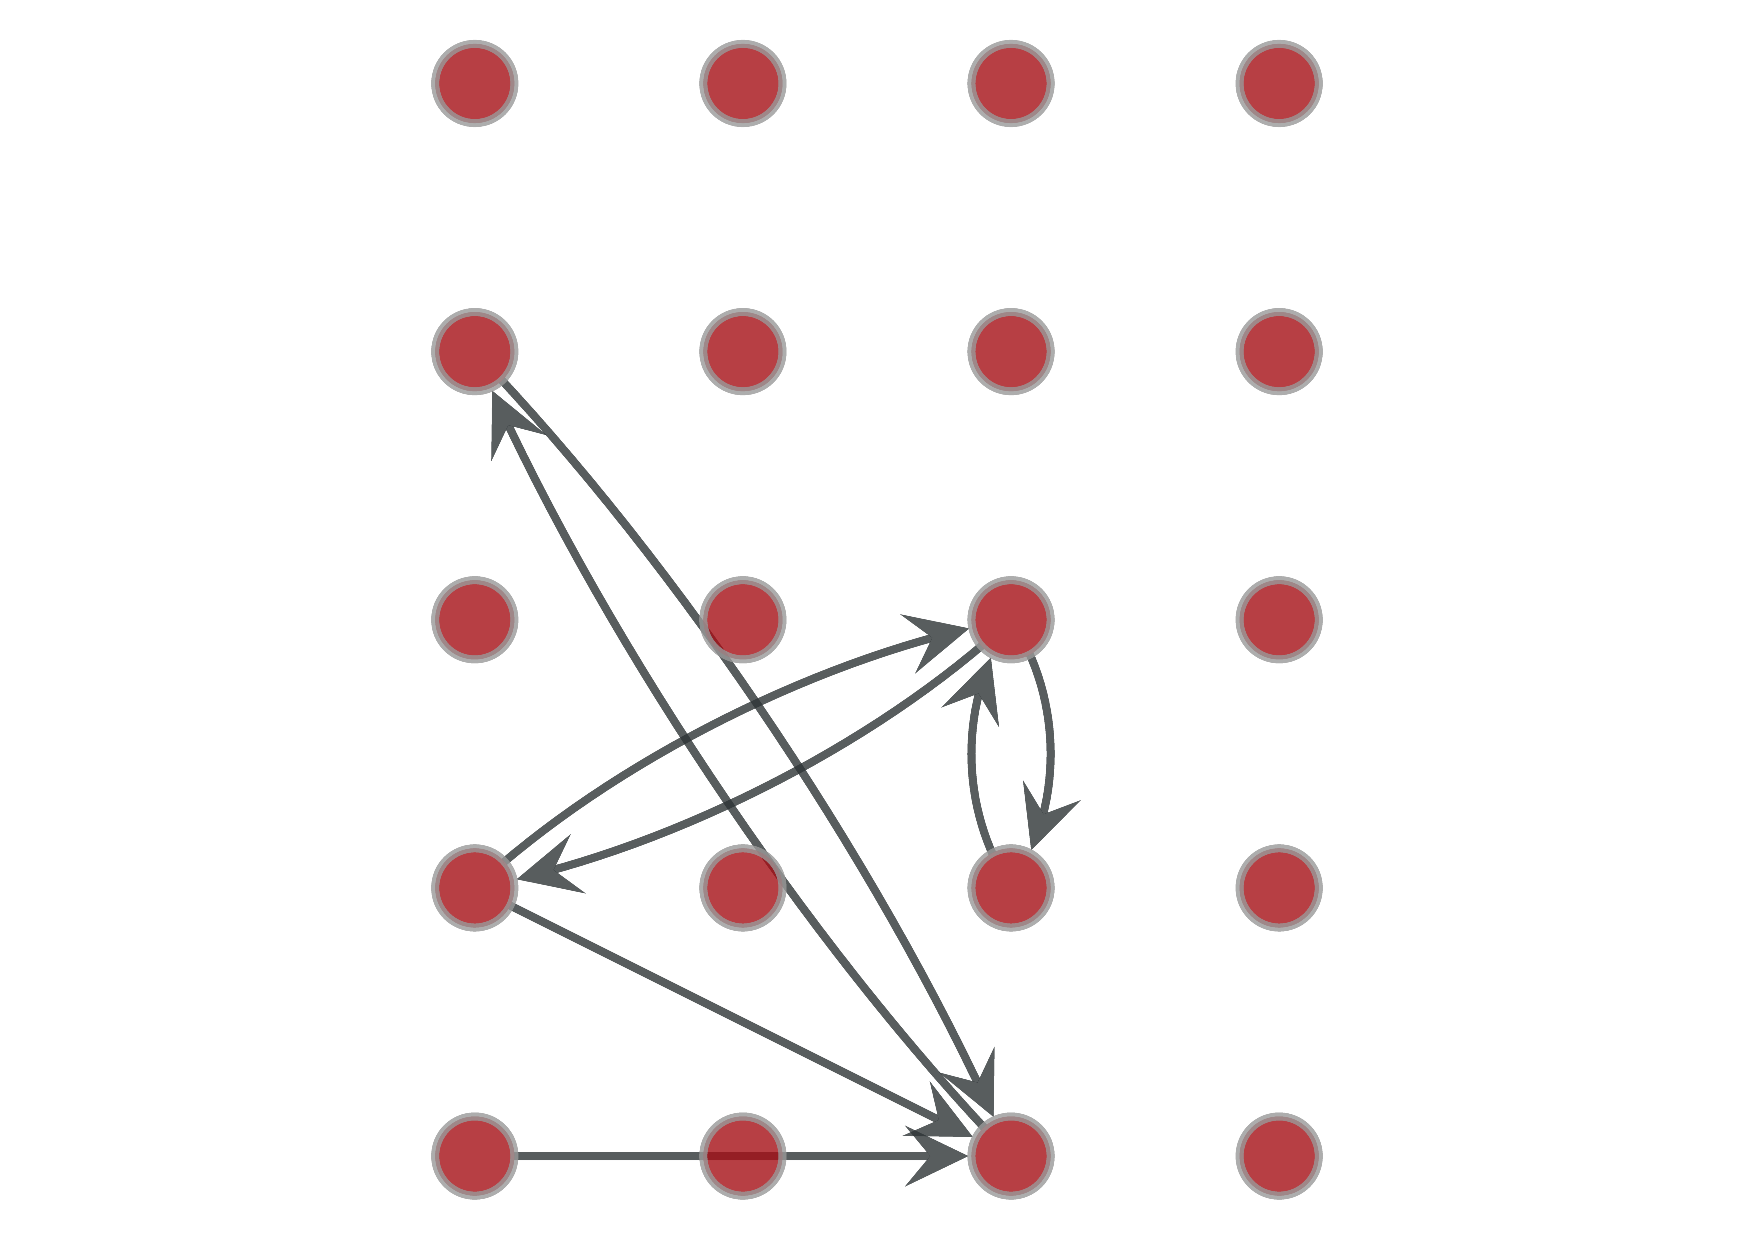
\includegraphics[height=4cm]{\MyPath/fig/2_firsthalf_.pdf}
		\caption{{\textbf{user 2}: 1\textsuperscript{st} half of the \mbox{observation period}}}
		\label{fig:evidence21}
	\end{subfigure}
	\begin{subfigure}[]{0.495\textwidth}
		\centering
		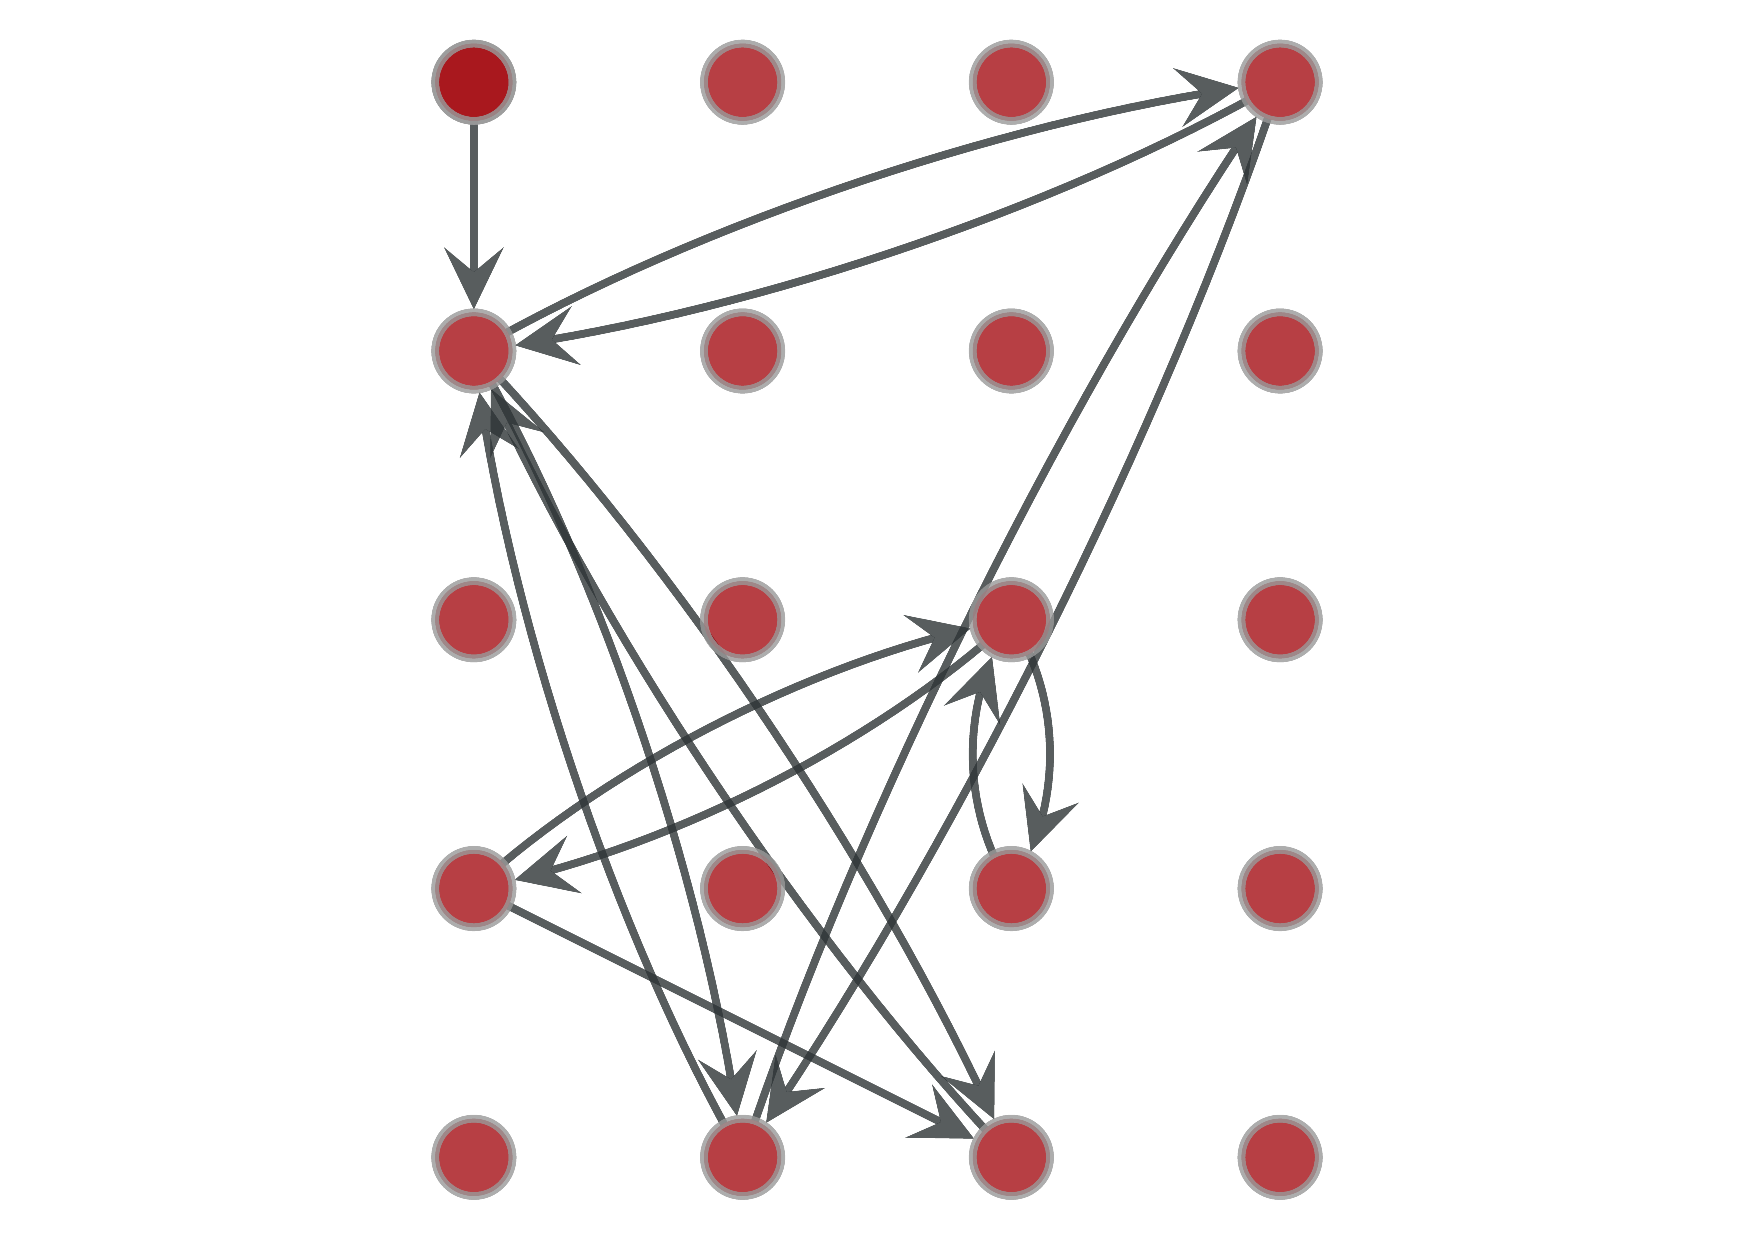
\includegraphics[height=4cm]{\MyPath/fig/2_secondhalf_.pdf}
		\caption{{\textbf{user 2}: 2\textsuperscript{nd} half of the \mbox{observation period}}}
		\label{fig:evidence22}
	\end{subfigure}
	\caption{{Top$-20$ networks for two random users from the Device Analyzer dataset.
			Depicted edges correspond to the highest $10$-th percentile of frequent transitions in the respective observation window.
			The networks show a high degree of similarity between the mobility profiles of the same user over the two observation periods.
			Moreover, the presence of single directed edges in the profile of \textbf{user 2} forms a discriminative pattern that allows us to distinguish \textbf{user\;2} from \textbf{user 1}.}}
	\label{fig:evidence}
\end{figure}

The basic premise of our deanonymization approach can be postulated as follows:

\emph{
	The mobility of a person across different time periods is stochastic, but largely recurrent and stationary, and its expression at the level of the individual mobility network is discriminative enough to reduce a person's privacy within a population.}

For example, the daily commute to work corresponds to a relatively stable sequence of cell towers.
This can be expressed in the mobility network of the user as a persistent subgraph, and forms a characteristic behavioural pattern that can be exploited for deanonymization of mobility traces.
Empirical evidence for our hypothesis is shown in~\cref{fig:evidence}.
For ease of presentation, in the figure, nodes between the disparate observation periods of the users can be cross-referenced. We assume that cross-referencing is not possible in our attack scenario, as locations are independently pseudonymized.


\subsubsection{Threat model \label{sec:threat-model}}

We assume that an adversary has access to a \emph{set of mobility networks} $ G \in \mcG_{\text{training}} $ \emph{with disclosed identities (or labels)} $l_{G} \in \mcL$
and a \emph{set of mobility networks} $ G' \in \mcG_{\text{test}} $ \emph{with undisclosed identities}
$ l_{G'} \in \mcL$.%

{Generally we can think of $ l_{G'} \in \mcJ \supset \mcL$ and assign some fixed probability mass to the labels $ l_{G'} \in \mcJ \setminus \mcL$.
However, here we make the \emph{closed world assumption} that the training and test networks come from the same population.
We make this assumption for two reasons: first, it is a common assumption in works on deanonymization and, second, we cannot directly update our beliefs on $ l_{G'} \in \mcJ \setminus \mcL$ by observing samples from $ \mcL$. }

We define a normalised similarity metric among the networks $ K: \mcG_{\text{training}} \times \mcG_{\text{test}} \rightarrow \mcR^+ $.
We hypothesize that a training and test mobility network belonging to the same person have common or similar connectivity patterns, thus a high degree of similarity.

The intention of an adversary is to deanonymize a given test network $ G' \in \mcG_{\text{test}} $, by appropriately defining a vector of probabilities over the possible identities in $ \mcL$.

An \textbf{uninformed adversary} has \emph{no information} about the networks of the population and, in the absence of any other side knowledge, the prior belief of the adversary about the identity of $ G' $ is a uniform distribution over all possible identities:
\[
	P\left(l_{G'}= l_{G_i}\right) := 1/|\mcL|, \mbox{ for every }  G_i \in \mcG_{\text{training}}.
\]

An \textbf{informed adversary} has \emph{access to the population of training networks} and can compute the pairwise similarities of $ G' $ with each $ G_{i} \in \mathcal{G}_{\text{training}} $ using a kernel function $K$. Hence the adversary can update her belief for the possible identities in $ \mathcal{L} $ according to the values of $K$.
Therefore, when the adversary attempts to deanonymize identities in the data, she assigns probabilities that follow a \emph{non-decreasing function} {of the computed pairwise similarity} of each label.
Denoting this function by $f$, we can write the updated adversarial probability estimate for each identity as follows:
\[
	P_K\left(l_{G'} =l_{G_i}| \mcG_{\text{training}}\right) :=  \frac{f\left(K(G_i, G')\right)}{\displaystyle \sum_{j\in \mcL}  f\left(K(G_j, G')\right)},   \mbox{ for every }  G_i \in \mcG_{\text{training}}.
	\label{eq:adversarial_rule}
\]




\subsubsection{Privacy loss}

In the case of the uninformed adversary, the true label for any user is expected to have rank $ |\mcL|/2$. Under this policy, the amount of privacy for each user is proportional to the size of the population.

In the case of the informed adversary, knowledge of $ \mcG_\text{training} $ and the use of $ K $ will induce some non-negative \emph{privacy loss} which will result in the expected rank of user to be smaller than $ |\mcL|/2$. The privacy loss ($\mathsf{PL}$) can be quantified as follows:
\[
	\mathsf{PL}\left(G';\mcG_{\text{training}}, K\right) := \frac{P_K\left(l_{G'}= l_{G'_\text{true}}|\mcG_{\text{training}}\right)}{P\left(l_{G'}= l_{G'_\text{true}}\right)} -1
	\label{eq:privloss}
\]

A privacy loss equal to zero reflects no information gain compared to an uninformed adversary with no access to graphs with disclosed identities.

Let us assume that the users of our population generate distinct mobility networks.
As will be supported with empirical evidence in the next section, this is often the case in real-world \emph{cid} datasets of few thousand users even for small network sizes (e.g. for top$-20$ networks in our dataset).
Under the above premise, the maximal privacy loss occurs when the presented test network is an identical copy of a training network of the same user which exists in the data of the adversary, \ie\ $ G' \in \mcG_\text{training}$.
This corresponds to a user deterministically repeating her mobility patterns over the observation period recorded in the test network.
In such a scenario, we could think that isomorphism tests are the most natural way to compute similarity; however, isomorphism tests will be useless in real-world scenarios, since, on top of their high computational cost, the stochastic nature and noise inherent in the mobility networks of a user would make them non-isomorphic.
Maximal privacy loss reflects the discriminative ability of the kernel and cannot be exceeded in real-world datasets, where the test networks are expected to be noisy copies of the training networks existing in our system.
The step of comparing with the set of training networks adds computational complexity of $O(|\mcG_{\text{training}}|)$ to the similarity metric cost.

Moreover, our framework can naturally facilitate incorporating new data to our beliefs when multiple examples per individual exist in the training dataset.
For example, when multiple instances of mobility networks per user are available, we can use $k-$nearest neighbors techniques in the comparison of distances with the test graph.
